\BiChapter{GPU计算}{performance}

上世纪六十年代提出的摩尔定律到目前为止已经持续了半个多世纪,硅技术似乎已经难以再有重大突破,摩尔定律在未来几年或将成为过去。然而当前计算机的计算能力仍不足以满足人们的需求,并行技术的发展在一定程度上缓解了这种压力,某种程度上而言,计算并行化可以看做是摩尔定律的一种延伸。

GPU(Graphic Processing Unit)又称“图形处理器”,是相对于CPU的一个概念,其最初目的是满足计算机图形界面中人们对于实时、高清的三维图形的需求。在图形开发中,由于图形渲染及变换等操作是带有可并行特征的,因此对于GPU的设计者而言,他们更倾向于添加更多的核心而不是提高核心的运行效率,通过多个核心以及线程技术,使得同一条指令可在每个元素上执行。此外,他们还取消了CPU中的缓存与逻辑控制部件,因此GPU适用于计算密集的并行计算,而CPU更适用于含有复杂流控的计算。

但是最初的GPU是为图形开发者而开发的平台,对于非图形开发者而言,使用GPU进行通用计算并不是一件容易的事。为此,ATI公司(已被AMD收购)于2005年提出的ATI Stream方案,NVIDIA公司在2007年推出的CUDA平台,都是为了解决GPU通用计算问题而做出的努力。在GPU通用计算不断发展的同时,新的规范也被不断地提出,Apple公司在2008年提出OpenCL(Open Computing Language)规范,微软提出的DirectCopmute规范,其目的都在于制定了一套API,并在此基础上开发GPU通用计算软件。

在这些GPGPU(General Purpose GPU)方案中,由于CUDA为开发者提供了一个类似于C的编程环境,使用者可以快速学习,所以受到了广泛的使用。


\BiSection{GPU体系结构}
x相比于CPU而言,GPU由于其设计原则就是针对密集运算的,所以在浮点运算上占着先天优势。近几年CPU在运算效率上的提升缓慢,与此同时,GPU计算却飞速发展,其运算性能已远远超过CPU。如图所示是Intel的CPU与NVIDIA的GPU在各个型号上每秒浮点运算量的对比。相比于CPU而言,GPU由于其设计原则就是针对密集运算的,所以在浮点运算上占着先天优势。近几年CPU在运算效率上的提升缓慢,与此同时,GPU计算却飞速发展,其运算性能已远远超过CPU。如图\ref{img:GPUvsCPU}所示是Intel的CPU与NVIDIA的GPU在各个型号上每秒浮点运算量的对比\footnote{图片出自于NVIDIA的官方技术文档《CUDA C Programming Guide》}。

\begin{figure}[!htbp]
\centering
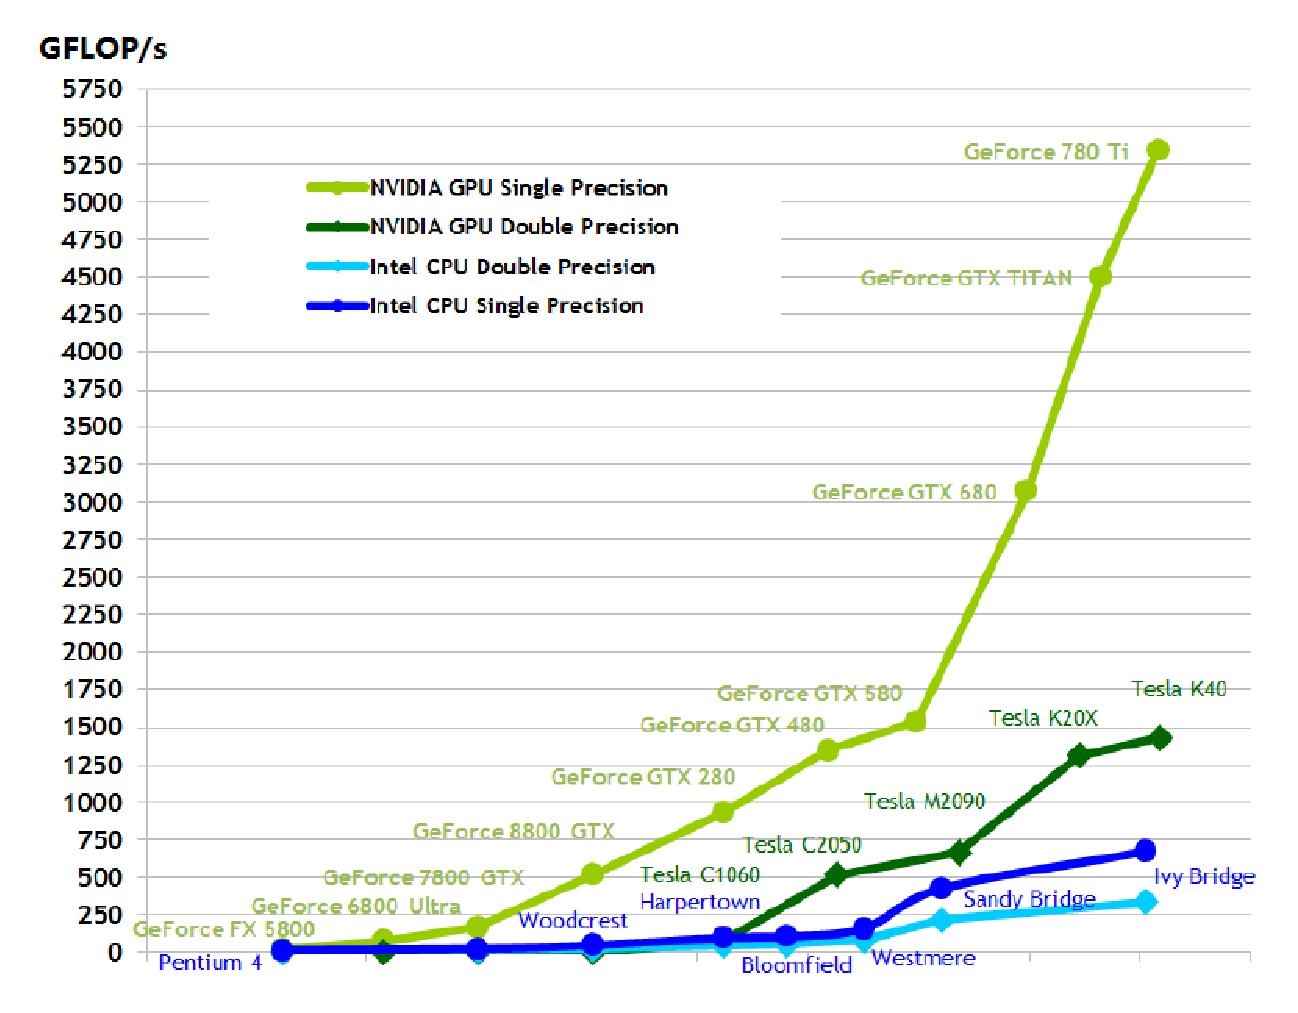
\includegraphics[width=0.57\textwidth]{GPU/GPUvsCPU.eps}
\caption{GPU与CPU在每秒浮点运算量上的差异}
\label{img:GPUvsCPU}
\end{figure}

由于GPU中取消了逻辑控制单元,相比于CPU其体系结构有着很大的不同。典型的CPU结构带有三级缓存,数据由内存经过三层缓存后才进入到处理器核心,这个结构如图所示。GPU同样带有缓存,这个缓存一般只有两级,与CPU不同的是,CPU中只有一个处理器,而GPU中并没有处理器核心的概念,取而代之的是流处理器簇(Streaming Muntiprocessor),在一个GPU中往往含有多个流处理器簇,尽管它们与CPU处理器核心有着很大的差异,但某种程度上也可以看做是GPU的核心,整个GPU的结构如图所示。

\begin{figure}[htbp]
\centering
\subfigure{\label{img:CPU}}\addtocounter{subfigure}{-2}
\subfigure{\subfigure[CPU结构]
			{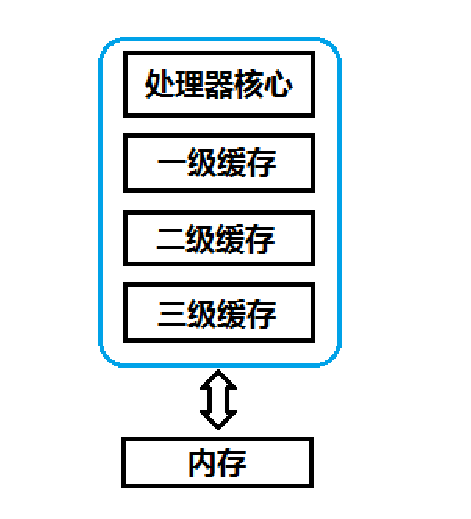
\includegraphics[width=0.32\textwidth]{GPU/CPU.eps}}}
\subfigure{\label{img:GPU}}\addtocounter{subfigure}{-2}
\subfigure{\subfigure[GPU结构]
			{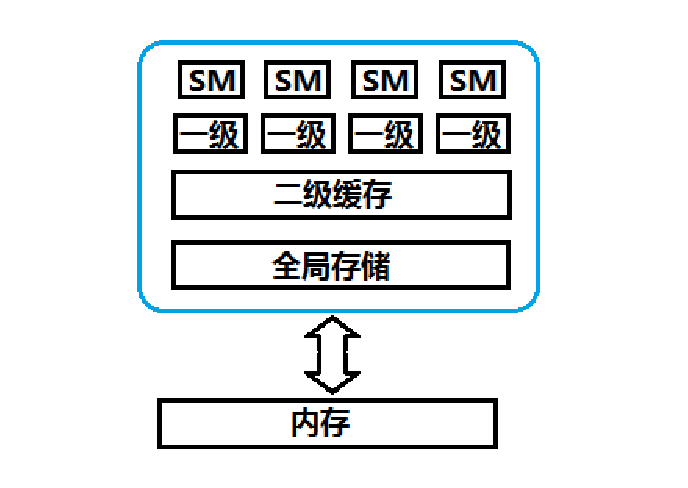
\includegraphics[width=0.46\textwidth]{GPU/GPU.eps}}}
\caption{CPU与GPU结构差异}
\vspace{-1em}
\end{figure}

CPU为了实现多核技术,往往在一个芯片中集成多个CPU核心,例如在Intel i7处理器中含有4个CPU核心,多核心使得CPU可以并行执行计算,但相比于GPU而言,CPU的并行粒度是非常大的。例如要将一个含有100个元素的向量的每一个元素乘上一个常数2,那么对于4核的CPU,我们可以指派1号CPU执行第1$\sim$25个元素的操作,2号CPU执行第26$\sim$50个元素的操作,但对于GPU而言,它可以直接开辟100个线程,每个线程针对每个元素进行操作,这些线程是并行线程而不是并发线程,因此GPU可以实现小粒度的并行。

GPU只所以能开辟大规模线程是因为一个GPU包含了一个流处理器簇阵列,这个阵列由多个流处理器簇构成,例如费米架构的GPU的阵列大小为16。而每个流处理器簇又包含了几十个到几百个的CUDA核心,例如,采用开普勒架构的GPU每个流处理器簇包含48个CUDA核心,而采用费米架构的GPU每个流处理器簇包含192个CUDA核心。这些核心并不类似于CPU的核心,CPU的每个核心只能执行一个线程,而CUDA核心可以并行执行多个线程。

GPU的线程由线程网格管理,线程网格可以看做是一个二维网格,这个结构如图\ref{img:thread grid}所示。在这个网格中,一个维度是线程块,另一个是线程束。每个GPU核心最多可包含65536个线程块,每个线程块最多可包含512个线程束,这意味着我们可以一次开辟最多大约3300万个线程,目前的费米架构已经实现每个线程块可包含1024个线程束,因此它最多可开辟6600万个线程。但这只是说我们可以在代码中开辟线程,并不意味着执行线程也是这个数量级。事实上,每个流处理器簇可执行的线程数量是有限制的,这个数量级大约是一千左右。

\begin{figure}[!htbp]
\centering
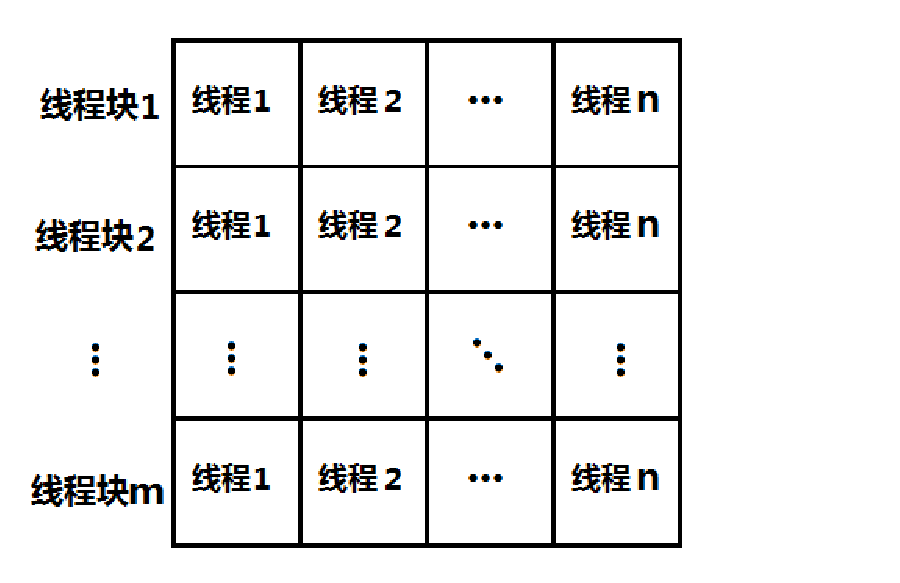
\includegraphics[width=0.6\textwidth]{GPU/threadGrid.eps}
\caption{线程网格}
\label{img:thread grid}
\end{figure}

实际中在跑的线程数大约为几万,然而我们却可以在代码中开辟几千万的线程,这得益于GPU对硬件的隐藏机制,类似于操作系统的虚拟地址,GPU会自动地将这几千万的虚拟线程在几万实际线程中调度,而程序员不需要参与到这个过程中,只需要在代码中开辟线程即可。这个机制使得硬件升级扩展变得简单,因为虚拟的线程与实际调度的线程是分离的,GPU为我们自动调度,我们可以随意的更换未来更多核心的GPU而不需要改动我们的代码。

为了更好地理解线程块与线程的概念,我们举一个GPU中实现两个向量相加的例子,如代码8.1所示

\begin{lstlisting}[language=C, numbers=left, frame=shadowbox, rulesepcolor=\color{cadegrey}, caption=\text{向量加法内核函数}]
__global__ void add(int *c, int *a, int *b){
	int tid = blockId.x;
	c[tid] = a[tid] + b[tid];
}
\end{lstlisting}

代码8.1中的的\_\_ kernel\_ \_ 代表这是一个在GPU中执行的代码,我们称其为内核函数。由\_\_ kernel\_\_ 标记的代码将由nvcc编译器编译,而没有这个标记的函数将由C++的编译器编译\footnote{例如Windows操作系统下的msvc或Linux操作系统下的gcc}。第2行代表获取当前的线程号,这里我们假定线程号就是线程块的编号,即默认每个线程块只有一个线程在运行。如果每个线程块有多个个线程在执行,那么第2行代码应改为

\begin{lstlisting}[language=C, frame=shadowbox, rulesepcolor=\color{cadegrey}]
int tid = threadIdx.x + blockId.x + blockDim.x;
\end{lstlisting}

观察图\ref{img:thread grid},这实质上类似于二维索引空间转换为线性空间的代码。代码8.1中的第3行代表每个线程执行一个操作,即将向量a中的第tid个元素与向量b中的第tid个元素相加,并存储在向量c的第tid个元素中。这可以理解为,代码8.1会做为一个副本分发给各个线程,各个线程拿到这段代码后,根据自己的线程ID(即tid)执行向量a和向量b中的第tid的元素的操作。


\BiSection{CUDA}
xCUDA(Compute Unified Device Architecture)是NVIDIA公司在2007年推出的高性能运算平台,它可以让GPU在执行常规的图形渲染的基础上额外地实现高性能的通用并行计算。CUDA包含了CUDA指令集架构以及GPU内部的并行计算引擎,通过利用 GPU 的处理能力,可大幅提升计算性能。支持CUDA平台的GPU包括NVIDIA Tesla 、NVIDIA Quadro 以及NVIDIA GeForce多个系列,其价格也涵盖了高端到底端多个市场,使得CUDA能够满足从消费级到专业级等多个方面的需求。目前为止, CUDA已经应用到图像与视频处理、计算生物学、流体力学模拟、金融风险分析、地震分析等多个领域,全球五百强企业以安装700多个基于CUDA的GPU集群,这些公司包括了能源领域的斯伦贝谢与雪佛龙以及银行业的法国巴黎银行等。

在CUDA中,程序员需要手工将数据从内存中迁移到GPU中,还需要负责GPU内存的回收,例如,为了执行两个向量的加法,其片段如代码8.2所示

\begin{lstlisting}[language=C, numbers=left, frame=shadowbox, rulesepcolor=\color{cadegrey}, caption=\text{GPU中向量加法的调用过程}]
int a[N], b[N], c[N];
int *dev_a, *dev_b, *dev_c;
//init a[N], b[N].....
cudaMalloc((void**)&dev_a, N*sizeof(int));
cudaMalloc((void**)&dev_b, N*sizeof(int));
cudaMalloc((void**)&dev_c, N*sizeof(int));
cudaMemcpy(dev_a, a, N*sizeof(int),cudaMemcpyHostToDevice);
cudaMemcpy(dev_b, b, N*sizeof(int),cudaMemcpyHostToDevice);
add<<<N, 1>>>(dev_c, dev_a, dev_a);	
cudaMemcpy(c, dev_c, N*sizeof(int),cudaMemcpyDeviceToHost);
cudaFree(dev_a);
cudaFree(dev_b);
cudaFree(dev_c);
\end{lstlisting}

在代码8.2中,我们先在GPU中申请内存,即对应的4$\sim$6行,随后在7$\sim$8行中将内存中的数据迁移到之前申请的GPU内存中。第9行执行代码8.1实现的加法内核函数,在GPU中开辟N个线程块,每个线程块含有1个线程,GPU完成计算后,我们在第10行将计算结果从GPU中迁移回内存,最后第11$\sim$13行释放之前申请的内存。释放内存是重要的,如果申请了内存不释放便会导致内存泄露,当内存消耗完毕后程序崩溃。

我们不由感叹,为了执行一个简单的向量加法就要编写如此多的代码,我们需要手工申请内存,手工将数据迁移到GPU中,手工调用内核函数,调用完毕后需要手工将计算结果从GPU中迁移回来,最后还需要手工释放申请的内存。如果用户不是专业的程序员,那么代码编写的过程十分困难。因此,在CUDA之上有多个团队为机器学习研究人员开发了专门的第三方库,我们将会介绍几个常见的包。
\BiSection{Cudamat}
xCudamat是一个由多伦多大学开发的一套针对于Python的开源第三方库\citeup{cudamat},它基于CUDA,在实现GPU高性能计算的同时保留了Python“语法优雅”的特性,所以使用者可以很方便地在Python语法层次上调用矩阵运算库。开发Cudamat的目的是为了方便机器学习建模,使科研人员从繁琐的CUDA编程中解放出来,由于GPU在浮点并行运算上巨大的优势,所以在计算密集的矩阵运算任务中Cudamat相对于numpy或MATLAB,其运算速度大约提升了50倍左右。

在Cudamat中,开发者已为我们重载了一些运算符,这使得矩阵的四则运算运算以及面向元素的四则运算,以及矩阵的切片、转置等操作不再需要编写大量的代码或调用对应的函数。此外,开发者还提供了一些常用的函数,例如面向元素的exp()、log()、sqrt()、pow(),矩阵的乘法以及面向轴的求和、随机矩阵的生成等。例如,为了实现一个logistic函数,只需要在Python中只书写代码8.3中的语句

\begin{lstlisting}[language=Python, frame=shadowbox, rulesepcolor=\color{cadegrey}, caption=\text{Cudamat中logistic的实现}]
def logistic(A):
   expTerm = cudamat.CUDAMatrix(numpy.random.randn(A.shape))
   cm.exp(-A, target=expTerm)
   return 1 / (1 + expTerm)
\end{lstlisting}

尽管Cudamat并没有将CUDA的所有功能都囊括其中,但在机器学习中常用的功能基本都实现了,所有我们可以在不需要了解底层CUDA的前提下高效地建立数学模型的代码,减轻了我们的工作量。


\BiSection{Gnumpy}
x在Python科学计算中,numpy与scipy两个第三方包充当着重要角色,其中numpy凭借其优美的语法实现以及高效地执行速率深受人们喜爱。在numpy中,有着许多巧妙的设计,比如广播特性、切片、方便的元素存取、丰富的函数等。其语法特性与MATLAB接近,几乎MATLAB上能实现的功能在numpy中都能找到对应的实现,此外还加入一些MATLAB所不支持的功能,例如方便地嵌入C++代码、方便地存储图像、网络IO等功能。尽管numpy语法简单,运行效率接近于C,但由于其本质上还是基于CPU的运算,所以在大规模的计算中运行效率显得有些难尽人意。

在Cudamat上编写代码要比直接地使用CUDA编写代码要方便得多,我们不再需要了解底层,不再需要担心GPU的内存释放,不再需要编写复杂的内核函数,然而,Cudamat代码要比numpy代码逊色不少,例如代码8.3中的exp函数需要在参数列表中带上返回变量,而这个返回变量又必须要先声明,无法实现变量的动态使用,所以Cudamat带着明显的C语言风格,这违背了Python关于“简单就是美”的设计原则。鉴于以上原因,多伦多大学在cudamat的基础上开发了新一代的开源第三方包---Gnumpy\citeup{gnumpy}。Gnumpy其计算本质是GPU计算,但其接口特性接近于numpy。尽管Gnumpy是基于Cudamat的,但在Gnumpy中你将看不到Cudamat的影子,开发者已经将其隐藏了,你看到的只有类似于numpy那样便捷的接口	。例如,同样是实现logistic函数,在Gnumpy中只需写成代码8.4中的形式

\begin{lstlisting}[language=Python,  frame=shadowbox, rulesepcolor=\color{cadegrey}, caption=\text{Gnumpy中logistic的实现}]
def logistic(A):
   return 1 / (1 + gnumpy.exp(-A))
\end{lstlisting}

事实上,gnumpy已经为我们实现了logistic函数,因此我们只需要一条语句即可完成该功能
\begin{lstlisting}[language=Python, frame=shadowbox, rulesepcolor=\color{cadegrey}]
A.logistic()
\end{lstlisting}

使用Gnumpy更容易编写程序,代码相对于Cudamat而言更简短,也更容易阅读与调试,对于拥有numpy使用经验的开发者而言可以很容易地上手。尽管Gnumpy是基于Cudamat的基础上进行的二次开发,但其运行效率接近于Cudamat,因此使用者无需过于担心效率问题。

\BiSection{PyCUDA}
x无论是Gnumpy或是Cudamat都只提供了一些矩阵的基本操作,我们无法实现一些这两个库没有的矩阵操作,例如二维离散卷积。如果我们因为内存管理的原因不想直接写繁琐的CUDA C代码,那么PyCUDA是一个可以选择的库。PyCUDA是由Andreas Klockner与Nicolas Pinto等人开发的一个Python第三方库\citeup{kloeckner_pycuda_2012},其目的在于允许我们在Python中内嵌CUDA C代码。在PyCUDA中,我们可以只书写内核函数,而不写内存管理的代码。在程序第一次执行时,Python会调用CUDA的编译器将CUDA C的代码编译成动态链接文件,编译完成后可以直接在Python中调用这个函数。例如,为了实现一个矩阵相乘的函数,我们的代码如代码8.5所示

\newpage
\begin{lstlisting}[language=Python,numbers=left, frame=shadowbox, rulesepcolor=\color{cadegrey}, caption=\text{Pycuda中实现向量相加}]
import pycuda.driver as GPU
from pycuda.compiler import SourceModule
def add(A, B, N):
    code = SourceModule('''
       __global__ void add(int *c, int *a, int *b){
          int tid = blockId.x;
          c[tid] = a[tid] + b[tid];
       }
    ''')
    addByGPU = code.get_function("add")
    C = numpy.zeros_like(A)
    addByGPU(GPU.Out(C), GPU.In(A), GPU.In(B),
             block=(N, 1, 1), grid=(1, 1))
    return C
\end{lstlisting}

代码8.5的第4$\sim$9行通过字符串的形式嵌入CUDA C的内核函数,第10行试图去获取名为“add”的内核函数,如果这行语句是第一次执行,并且在我们已经通过字符串形式嵌入了“add”这个函数,那么Python就会调用nvcc编译器对代码进行编译,并保存为动态链接文件,当下一次再试图获取这个内核函数时不需要再编译一次而直接调用。第$12$行执行GPU中的计算,以A、B作为输入,C作为输出,执行在N个线程块上。最后返回运算结果C。

PyCUDA使得我们的代码自由度变得更高,我们可以实现任何一个我们想要的内核函数。但与此同时它也使得我们的代码变得复杂。天下没有免费的午餐,选择一个自由度高的库或是选择一个代码简单的库完全取决于你的权衡。

\BiSection{Caffe}
x以上的几个Python第三方库都是一些机器学习中的通用库,这些库只提供基础的功能,利用他们可以实现很多算法。如果一个科研人员没有太多程序设计的经验,而又希望将他设计的神经网络在计算机上实现,那么Caffe是一个选择。Caffe是由加州大学伯克利分校的Jia Yangqing 等人的领导下开发的一套基于CUDA的深度学习工具箱\citeup{jia2014caffe},其源代码由C++/CUDA实现,在此之上提供了Python、MATLAB接口,并且可以通过命令行执行。在Caffe中,开发者已经编写好各种各样的网络层的代码,如全连接层、卷积层等。使用者无需编写具体的代码,Caffe让深度学习的研究人员从具体的代码中解放出来,我们只需要将自己设计的网络模型写成配置文件即可。如代码8.6是一个神经网络的配置文件中的一个片段

\begin{lstlisting}[language=Python,numbers=left, frame=shadowbox, rulesepcolor=\color{cadegrey}, caption=\text{神经网络配置文件片段}]
layers {
    name: "pool1"
    type: POOLING
    bottom: "conv1"
    top: "pool1"
    pooling_param {
        pool: MAX
        kernel_size: 3
        stride: 2
    }
}
\end{lstlisting}

在代码8.6的配置文件片段中,定义了一个池化层。配置文件由两部分组成,2$\sim$5行为属性定义,6$\sim$10行为参数定义。其中第2行定义了这层的名字,第3行定义了层的类型,第4行定义了这层网络的前一层网络的名字,第5行定义了后一层网络的名字(这里就是它自身)。第7行定义了这层池化层使用的是最大池采样,第8行定义了卷积核的尺寸为$3\times 3$,第9行定义了卷积间隔为2。



\BiSection{本章小结}
x本章中,我们介绍了GPU计算,由于本文并不是一个GPU编程指南,因此我们仅限于简单地介绍,更多关于CUDA C的编程指南可参考文献\cite{CUDA}和\cite{CUDAcode}。在本章的后半阶段,我们介绍了几个基于CUDA开发的库,关于这几个库如何选取,如果需要编写的代码只含有简单的矩阵操作,那么我们推荐使用Gnumpy库,如果代码中含有一些很复杂的矩阵操作,而这些操作又是可并行的,那么我们推荐使用PyCUDA。这两个库除了可以用在神经网络中外还可以用在别的机器学习算法上,因为它们提供的功能是如此的基础以至于你可以任意组合出你希望的代码。如果工作的内容只涉及神经网络,而又不想编写代码,那么我们推荐使用Caffe。



